% 01/10/2025

\chapter{Introduzione al corso}
\section{Organizzazione}
\par In più rispetto all'ultimo semestre:
\begin{itemize}
    \item "gettoni presenza" per punti bonus
    \item 15 ottobre: conferenza azienda (BendingSpoons) su iOs
\end{itemize}

\section{Obiettivi del corso}
\par Il corso ha come obiettivo acquisire:
\begin{itemize}
    \item \textbf{\underline{Conoscenze}} (principi di buona programmazione) relative al mondo dello sviluppo mobile
    \item \textbf{\underline{Competenze}} sullo sviluppo Android 
\end{itemize}
\par Ma perché è stato scelto proprio Android? Comporta diversi vantaggi rispetto ad altri sistemi operativi come iOs:
\begin{itemize}
    \item più open source
    \item essendo più open source conosciuto meglio dai docenti che sono quindi più in grado di insegnare e correggere
    \item Android, nel caso uno voglia poi accedere allo Store e pubblicare un'app, prevede una tassa di iscrizione di \texttildelow 25\$ \textbf{una tantum}, mentre per iOs è di 100\$ ma penso sia \textit{annuale}.
\end{itemize}
\par Alla fine del corso dovremo essere in grado di:
\begin{itemize}
    \item Sviluppare un'applicazione ``from scratch'' che segua l'\textbf{\underline{architettura}} di riferimento Android
    \begin{itemize}
        \item alla fine se abbiamo rispettato o no l'architettura presentata a lezione è quello che guardano di più della nostra app, se non è bellissima o funzionante al 101\% importa meno
    \end{itemize}
    \item Comprendere il funzionamento di applicazioni Android
\end{itemize} 

\section{Il corso in pillole}
\begin{enumerate}
    \item \textbf{Introduzione} alla progettazione e allo sviluppo di applicazioni mobili
    \item \textbf{Linee guida} sull'architettura dell'app
    \item \textbf{Sviluppo} di un'app in Java\\
    Per il nostro progetto possiamo usare Java o Kotlin, la teoria rimane la stessa, ma a lezione useremo solo Java. Questo perché è già stato presentato ed usato in altri due corsi e quindi conosciuto meglio da docenti e studenti. Inoltre, è previsto (penso in entrambi i linguaggi) l'uso di lambda functions, più elegante e funzionale in Kotlin, però buono anche in Java. Infine, Java risulta più conveniente per l'uso di librerie esterne di Kotlin, che è più giovane e meno conosciuto e quindi ha meno librerie disponibili.\\
    Eventualmente, sul sito Google ci sono disponibili diversi tutorial gratuiti (video) per imparare Kotlin e per la migrazione del mio progetto da Kotlin a Java.\\
    Se si vuole utilizzare Kotlin, c'è da scrivere alla professoressa spiegando le ragioni della scelta.\\
    L'app deve essere robusta. La robustezza si basa sull'autonomia dalla connessione di rete. Il concetto ``\underline{offline-first}'' è molto importante, prima di tutto l'app deve funzionare senza connessione. Inoltre, deve essere anche \underline{evolvibile}. Oltre ai suoi componenti funzionali (ovvero le sue \underline{funzionalità}) di base, ci sono determinate funzionalità che devono essere mantenute ed evolute/ampliate nel tempo.\\
    La nostra app deve essere:
    \begin{enumerate}
        \item Compliant con l'architettura di riferimento\\
        La cosa \underline{importante} della nostra app non è l'estetica o se funziona bene, ma \textbf{\underline{come}} l'architettura presentata a lezione viene sviluppata.
        \item Con UI
        \item Che accede alla rete per i dati (API esterne)
        \item Che fa persistenza (\underline{locale + remoto})\\
        Ovvero deve funzionare \textit{localmente} e salvare localmente i dati (importante per il concetto di ``\textit{offline-first}''). Però deve anche salvare \textit{in remoto} i dati, ma deve rispettare la \textit{cross-device synchronization}.\\
        Importante per quanto riguarda la \underline{cross-device synchronization}, ovvero deve funzionare su diversi dispositivi con stato sincronizzato.
        \item Che usa Firebase\\
        Firebase è un framework di Google che offre una serie di servizi per lo sviluppo di applicazioni mobili.
    \end{enumerate}
\end{enumerate}

\section{Il progetto}
\begin{itemize}
    \item Durante il corso si porta avanti un progetto che sarà oggetto dell'esame finale
    \item Il progetto è svolto in maniera paritaria da un gruppo di studenti
    \begin{itemize}
        \item Composto da almeno 3 persone e fino ad un massimo di 5
        \item Eccezioni verranno valutate singolarmente
    \end{itemize}
    \item Il progetto è proposto dal gruppo (scadenza 17 ottobre 2025)
    \begin{itemize}
        \item L'idea può anche essere non nuova, ad esempio un'app che mostra i film e le recensioni\dots
    \end{itemize}
    \item Il progetto deve essere sviluppato per Android (in Java)
    \item \underline{Assistenza al progetto} (oltre che ai laboratori durante i quali lavoreremo sul \textbf{nostro} progetto) verrà fornita \textit{eventualmente} anche durante le \underline{esercitazioni} (durante le quali vedremo come realizzare un'applicazione da zero tramite un \textit{progetto} \underline{scelto dal docente} con le proprie funzionalità e sviluppato \textbf{\underline{esattamente}} come vuole la prof che sia realizzata la nostra app)
    \item Si suggerisce caldamente per chi voglia sfruttare l'appello invernale per sostenere l'esame di seguire i laboratori perché verrà fornita assistenza.
    \item L'app deve \textbf{NECESSARIAMENTE} avere:
    \begin{enumerate}
        \item architettura
        \item almeno 1 API esterna
        \item autenticazione se necessario
        \item off-line first (deve funzionare fluidamente anche in assenza di connettività)
        \item cross-device synchronization
        \item testing
        \item layout grafico (importante ma meno del resto)
        \item storage locale (opzionale: se necessario, ma ne va giustificata l'assenza in caso)
        \item documentazione di buona qualità (ci sono molti esempi sul drive presente su Moodle)
    \end{enumerate}
    \item Bisogna usare GitLab o GitHub (non per forza ma una settimana prima della consegna va fatto quindi tanto vale)
\end{itemize}

\subsubsection{Valutazione}
\begin{itemize}
    \item Codice sorgente e documentazione della nostra app con dentro:
    \begin{enumerate}
        \item Scelte architetturali
        \item Uso di API esterne (in maniera sensata)
        \item Uso storage locale, per offline-first
        \item Uso del framework Firebase (autenticazione), per cross-device synchronization
        \item Layout grafico che sia (circa) sensato, per es. tramite uso librerie di material design
        \item Documentazione
    \end{enumerate}
    \item Punti 1-5 chiaramente via Software, 6 cartaceo
    \item Uso di GitLab o GitHub (da aggiungere account fornito dai docenti)
\end{itemize}

\subsection{1. Scelte architetturali}
\begin{center}
    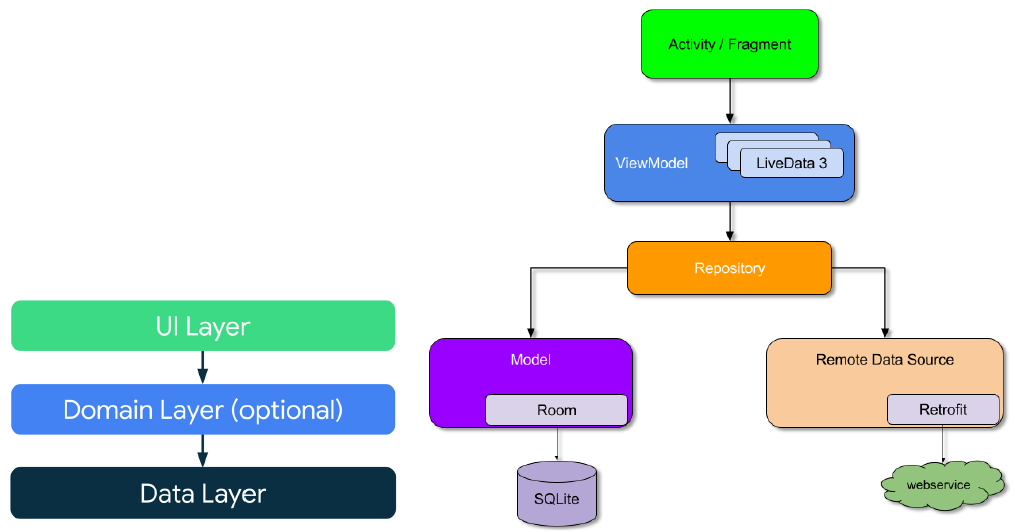
\includegraphics[width=0.5\textwidth]{images/00_scelte_architetturali1.png}
\end{center}
\par Queste 5 entità \textbf{\underline{devono}} essere presenti nel nostro progetto.

\subsection{2. Uso di API esterne}
\par Esempi di API esterne (gratuite):
\begin{itemize}
    \item Immagini
    \begin{itemize}
        \item \url{https://unsplash.com/developers}
        \item \url{https://developers.google.com/maps/documentation/places/web-service/photos}
    \end{itemize}
    \item Video Giochi
    \begin{itemize}
        \item \url{https://www.igdb.com/api}
    \end{itemize}
    \item Film
    \begin{itemize}
        \item Film
        \item MovieDB
        \item Open Moview DB
        \item IMDb
        \item The Moview DB
    \end{itemize}
    \item Qualità dell'aria
    \begin{itemize}
        \item \url{https://aqicn.org/}
    \end{itemize}
    \item Cibo
    \begin{itemize}
        \item TheMealDB.com
        \item \url{https://spoonacular.com/food-api}
    \end{itemize}
    \item Meteo
    \begin{itemize}
        \item \url{https://openweathermap.org/current}
    \end{itemize}
    \item …
\end{itemize}
\par Tante disponibili free
\begin{itemize}
    \item \url{https://github.com/public-apis/public-apis}
\end{itemize}
\par Postman è un'applicazione che permette di testare le API, di interrogarle, è molto utile per vedere come funzionano le API e come si comportano prima di integrarle. \url{https://www.postman.com/}

\subsection{3. 4. 5. Uso di Firebase}
\par Strumento molto potente, lo vedremo ad esercitazione. Ti aiuta a creare:
\begin{itemize}
    \item Autenticazione
    \begin{itemize}
        \item se necessario nell'app
    \end{itemize}
    \item Database remoto
    \begin{itemize}
        \item Anche a supporto della cross-device synchronization
    \end{itemize}
    \item Notifiche push
    \item \dots
\end{itemize}

\subsection{6. Testing}
\begin{itemize}
    \item JUnit 4/5
    \item Mockito/MockK
    \item Espresso (per test UI, con un input di testo e comandi per interagire con l'UI) !!!
    \item Robolectric
    \item Firebase Test lab
    \item UI Automator (quella che mi permette di fare il cross-app testing) !!!
\end{itemize}
Quelli con "!!!" sono quelli evidenziati dalla prof.

\subsection{7. Layout grafico}
\par Non una delle cose essenziali ma comunque importante, l'app deve comunque essere user-friendly.
\par Ho delle regole da seguire, il progetto deve seguire i principi di material design (che sono linee guida di Google per lo sviluppo di UI, ma ci sono anche widget grafici, gratuiti ed usabili). Per esempio: color extraction (tutti i widget hanno colorazione uniformata allo sfondo per conferire maggiore fluidità).
\begin{center}
    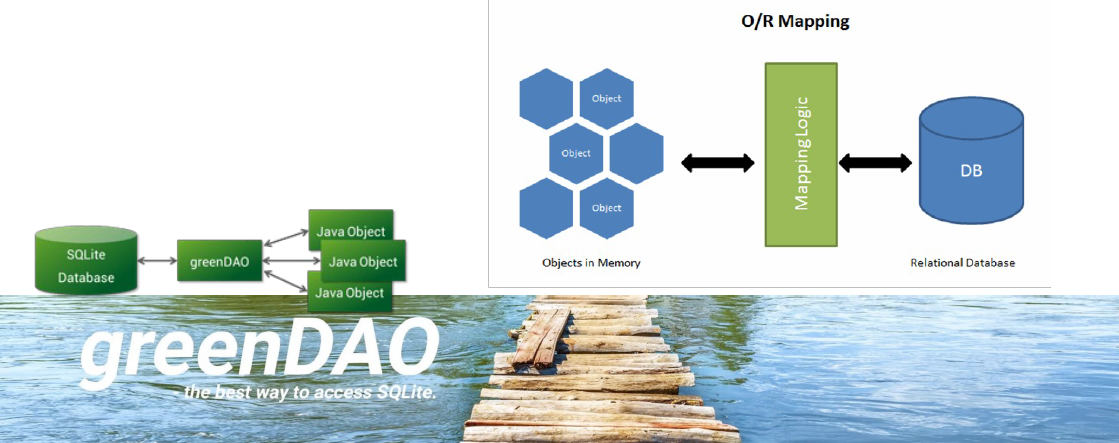
\includegraphics[width=0.5\textwidth]{images/00_orm1.png}
\end{center}

\subsection{8. Uso ORM - Object Relational Mapping}
\par Uso di ORM (Object-relational mapping). Due tool sono:
\begin{itemize}
    \item Room (integrato in Android), utile per persistenza
    \item greenDao, più vecchio ma ancora in uso
\end{itemize}

\subsection{Documentazione}
\par La documentazione dovrà essere strutturata in 3 sezioni:
\begin{enumerate}
    \item le \textbf{funzionalità offerte}
    \begin{itemize}
        \item potete scriverle in italiano, oppure usare degli use case
    \end{itemize}
    \item l'\textbf{architettura complessiva} che specifica i componenti da voi sviluppati e le loro relazioni e modalità di comunicazione con eventuali componenti esterni utilizzati
    \begin{itemize}
        \item Firebase, API esterne, DB interno, etc.
    \end{itemize}
    \item il \textbf{design della soluzione} che include i \textit{componenti} che avete sviluppato (inteso come Fragment, Activity, etc.), le loro \textit{responsabilità} (cioè cosa fanno) le loro \textit{modalità di interazione}
\end{enumerate}
\par Alcuni esempi, sul drive fornito dalla prof su Moodle.

% \subsection{Discussione progetto}
% \begin{itemize}
%     \item 24 gennaio 2025, \texttildelow 09:00
%     \item 21 febbraio 2025, \texttildelow 09:00
% \end{itemize}

\subsection{Scadenze}
\begin{itemize}
    \item \underline{10 ottobre 2025}: comunicazione gruppo
    \begin{itemize}
        \item la composizione del gruppo (matricola, cognome, nome), un nominativo per riga;
        \item il referente del gruppo.
    \end{itemize}
    \item \underline{17 ottobre 2025}: comunicazione argomento progetto
    \begin{itemize}
        \item Il titolo del progetto;
        \item una descrizione del progetto che si intende svolgere;
        \item il referente del gruppo.
    \end{itemize}
\end{itemize}

